%!TEX TS-program = xelatex
%!TEX encoding = utf8

%title: LaTeX-Standarddokument
%authors: Christian Müller, Nicolas Zahn
%last changed: 02.10.2011

\documentclass[paper=a4    % Papierformat
,twoside=false             % einseitiges Dokument
,fontsize=12pt             % Standard Schriftgrösse
,DIV=11                    % Grundraster für die Satzspiegelkonstruktion
,parskip=half		   % Einrücken nach Absatz wird deaktiviert
]{scrartcl}

%%%% Encoding %%%% (wenn nicht mit Xe\LaTeX{})
\usepackage[utf8]{inputenc}

%%%% Pakete, die nie fehlen dürfen %%%%
\usepackage{graphicx}      % für die Einbindung von Graphiken
\usepackage{tabularx}      % erweiterte Tabellenfunktionen
\usepackage{booktabs}      % für die schöne Darstellung von Tabellen
\usepackage{xcolor}        % für die Möglichkeit farbigen Texts

%%%% Sprache %%%%
\usepackage[ngerman]{babel}

%%%% Misc. Pakete %%%%
\usepackage{url}
\mathchardef\UrlBreakPenalty=100
\mathchardef\UrlBigBreakPenalty=100

%%%% Hyperlinks %%%%
\usepackage{hyperref}

%%%% Titelinformationen %%%%
\author{Nicolas Zahn}
\title{Beispieldokument}
\date{\today}

%%%%%%%%%%%%%%%%%%%
% Beginn Dokument %
%%%%%%%%%%%%%%%%%%%

\begin{document}
%Inhaltsverzeichnis erstellen: in \LaTeX{} ist dazu nur ein Befehl notwendig (h\"angt von der gew\"ahlten Sprache ab)
\tableofcontents
%Es lassen sich ganz einfach auch weitere Verzeichnisse erstellen, beispielsweise Abbildungs- und Tabellenverzeichnisse
\listoffigures
\listoftables
%ein neues Kapitel
\section{Text- und Absatzformatierung}
So sieht normaler Fliesstext in \LaTeX{}  aus. 
Zeilenumbr\"uche im Quellcode haben keinen Einfluss auf das gesetzte Dokument, stattdessen m\"ussen Umschl\"age mit zwei Backslashes erzwungen werden. \\
So geht das.
%ein neues Unterkapitel
\subsection{Textformatierung}
Hier schauen wir uns klassische M\"oglichkeiten der Textformatierung an, wie Schriftgr\"osse, fetten Text, kursiven Text etc.
%ein weiteres Unterkapitel, diesmal ohne Nummer (*)
\subsubsection*{Beispiele Schriftgr\"osse}
\tiny{winziger Text}\\
\small{kleiner Text}\\
\large{grosser Text}\\
\huge{riesiger Text}\\
\normalsize{Anmerkung: die Schriftgr\"osse \"andert sich durch die Befehle \texttt{tiny, large} etc. relativ zur standardm\"assig gesetzen Schriftgr\"osse (hier: 12pt).}
\subsubsection*{Beispiele Zeichensatz}
\textbf{fetter Text} (bold format)\\
\textit{kursiver Text} (italic)\\
\textsc{Kapit\"alchen} (small caps)\\
\emph{hervorgehobener Text} (emphasize, Besonderheit: wird dieser Befehl in einem bereits kursiven Text verwendet, wird automatisch aufrecht gesetzt)\\
\underline{unterstrichener Text}\\
Text \textsuperscript{hochgestellt} (alternativ: Text$^{hochgestellt mittels Formelumgebung}$)\\
Text \textsubscript{tiefgestellt} (alternativ: Text$_{tiefgestellt mittels Formelumgebung}$)
\subsection{Absatzformatierung}
Standardm\"assig wird in \LaTeX{} im Blocksatz gesetzt (meistens auch f\"ur Arbeiten Standard), Abweichungen sind dennoch m\"oglich.
\begin{center}
Zentrierter Absatz: Lorem ipsum dolor sit amet, consetetur sadipscing elitr, sed diam nonumy eirmod tempor invidunt ut labore et dolore magna aliquyam erat, sed diam voluptua.
\end{center}
\begin{flushright}
Rechter Absatz: Lorem ipsum dolor sit amet, consetetur sadipscing elitr, sed diam nonumy eirmod tempor invidunt ut labore et dolore magna aliquyam erat, sed diam voluptua.
\end{flushright}
\begin{flushleft}
Linker Absatz: Lorem ipsum dolor sit amet, consetetur sadipscing elitr, sed diam nonumy eirmod tempor invidunt ut labore et dolore magna aliquyam erat, sed diam voluptua.
\end{flushleft}
\begin{quote}
Einger\"uckter Absatz (z.B. langes Zitat): Lorem ipsum dolor sit amet, consetetur sadipscing elitr, sed diam nonumy eirmod tempor invidunt ut labore et dolore magna aliquyam erat, sed diam voluptua.
\end{quote}
Seitenumbruch: \newpage
Weiter gehts!
\section{Fussnoten und Verweise}
Fussnoten k\"onnen in \LaTeX{} ganz einfach mit dem Befehl \texttt{footnote} erzeugt werden\footnote{Nat\"urlich werden diese auch automatisch nummeriert.}. Die horizontale Linie ist dabei standardm\"assig aktiviert, l\"asst sich aber durch \texttt{renewcommand} unterdr\"ucken.\\
Verweise erfolgen indem zuerst ein Label gesetzt wird auf das Objekt, auf welches verwiesen werden soll (in diesem Beispiel dieser Absatz \label{test}): \\
Verweis: dieser Absatz steht im Kapitel \ref{test} auf Seite \pageref{test}.\\
\section{Aufz\"ahlungen und Listen}
Aufz\"ahlungen und Listen k\"onnen in \LaTeX{} nummeriert oder mit Symbolen erstellt werden. Ausserdem kann man sie verschachteln oder auf einzelne Listenelemente verweisen.
%nicht nummerierte Liste
\begin{itemize}
	\item ein Aufz\"ahlungspunkt mit dem Standardsymbol
	\item [*] ein Aufz\"ahlungspunkt mit Stern
	\item [-] ein Aufz\"ahlungspunkt mit Strich
\end{itemize}
%nummerierte Liste
\begin{enumerate}
	\item erster Listenpunkt
	\item zweiter Listenpunkt
	\item \dots
\end{enumerate}
%verschachtelte Liste mit Verweis
\begin{itemize}
	\item noch ein Aufz\"ahlungspunkt
	\item jetzt kommt ein Aufz\"ahlungspunkt mit Unterpunkten welche nummeriert werden sollen
	\begin{enumerate}
		\item Auto
		\item Fahrrad
		\item Zug \label{enum:zug}
	\end{enumerate}
	\item nochmals ein Aufz\"ahlungspunkt mit Unterpunkten ohne Nummerierung
	\begin{itemize}
		\item \dots
	\end{itemize}	
\end{itemize}
Der Zug steht unter Punkt \ref{enum:zug}.
\section{Tabellen und Bilder}
Tabellen und Bilder werden in \LaTeX{} am einfachsten in der sogenannten Float-Umgebung eingebunden. Das bedeutet, dass die Bilder und Tabellen so gesetzt werden, wie es vom Textfluss her am besten passt, was das punktgenaue Einf\"ugen dieser Objekte etwas erschwert. Allerdings k\"onnen manuell andere Umgebungen gesetzt werden (sog. \texttt{nofloat}).
\subsubsection*{Beispiele}
\begin{table}[h]
	\begin{tabular}{| c | l | l |}
		\hline
		\textit{Platz} & \textit{Name} & \textit{Zeit} \\
		\hline
		1. & X & 10.52 \\
		2. & Y & 12.34 \\
		3. & Z & 23.42 \\
		\hline
		\end{tabular}
	\caption{Eine einfache Rangliste}
\end{table}
\begin{table}[h]
	\begin{tabular}{ c  l  l}
		\hline
		\textit{Platz} & \textit{Name} & \textit{Zeit} \\
		\hline
		1. & X & 10.52 \\
		2. & Y & 12.34 \\
		3. & Z & 23.42 \\
		\hline
		\end{tabular}
	\caption{Eine einfache Rangliste (ohne seitlichen Rahmen)}
\end{table}
\begin{table}[h]
	\begin{tabular}{ c  l  l }
		\textit{Platz} & \textit{Name} & \textit{Zeit} \\
		1. & X & 10.52 \\
		2. & Y & 12.34 \\
		3. & Z & 23.42 \\
		\end{tabular}
	\caption{Eine einfache Rangliste (ohne Rahmen)}
\end{table}
\begin{table}[tb!]
	\begin{center}
		\begin{tabular}{@{}lr@{}}
		\toprule
		Variable 	&	Koeffizient\\ 
		& \emph{(t-Wert)} \\
		\midrule
		Konstante & 21.11*** \\
		($\alpha$) & \emph{(37.04)} \\
		Erfahrung & 0.13**\\ 
		($\beta_{1}$) & \emph{(2.18)}  \\
		ideologische Distanz & -0.43** \\
		($\beta_{2}$) &\emph{(-2.16)}  \\
		Erfahrung * ideologische Distanz & 0.05* \\
		($\beta_{3}$) & \emph{(1.72)}  \\ \hline
		Geschlecht &  1.38'\\
		($\beta_{4}$) &   \emph{(1.23)}  \\
		L\"ange der Wahlliste &   -0.06**\\
		($\beta_{5}$) &  \emph{(-2.54)}  \\ \midrule
		 $N$  & 134\\
		 $\bar R^{2}$ &  0.1320\\ 
		\bottomrule
		\multicolumn{2}{l}{\small{Signifikanzniveau: ': $ >$10\% *: 10\% **: 5\% ***: 1\%}}
		\end{tabular}
		\caption{Resultate der Regressionsanalyse;
		  \textit{Quelle(n)}: Kerr 1974, eigene Berechnungen.}
		\label{reg}
	\end{center}
\end{table}
\begin{figure}[t!]
	\begin{center}
		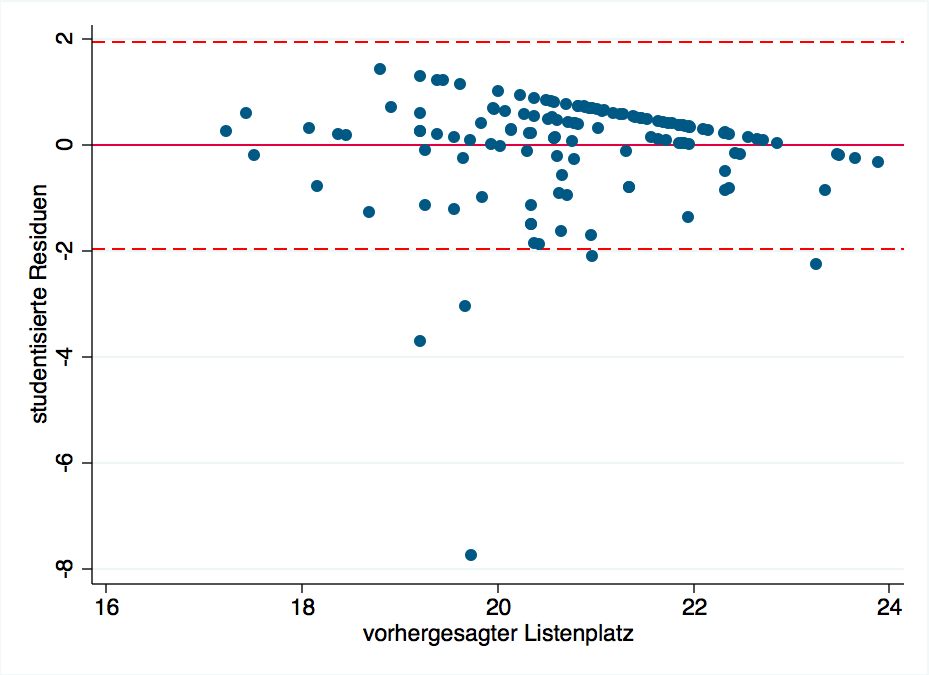
\includegraphics[width=15cm]{diag1.png}
		\caption{Graphischer Test auf Heteroskedastizit\"at.}
		\label{diag1}
	\end{center}
\end{figure}
\section{Formeln}
\end{document}
